\begin{frame}[t]{Where each first pass stopped}
\smallbody Each task appears once per arm. For a returned answer, the classification follows the saved query grids. For a missing answer, it follows the last recorded attempt and its saved text.
\par\vspace{2mm}
\begin{center}
\smallbody\renewcommand{\arraystretch}{.99}\begin{tabular}{@{}lrr@{}}
\toprule
Outcome at the snapshot & Arm A & Arm B\\
\midrule
Deadline before first completed candidate & 107 & 89\\
Prompt reached context limit before generation & 7 & 7\\
Completed response rejected as a solver or probe & 2 & 14\\
\addlinespace
At least one query grid missing & 1 & 0\\
All grids returned, wrong dimensions & 3 & 2\\
Right dimensions, returned input unchanged & 0 & 3\\
Right dimensions, changed cells, wrong answer & 4 & 5\\
Exact on every query & 0 & 1\\
\addlinespace
Started, still open & 6 & 7\\
No recorded attempt & 8 & 10\\
\midrule
\textbf{Held-out tasks} & \textbf{138} & \textbf{138}\\
\bottomrule\end{tabular}
\end{center}
\vfill
\smallbody All 18 wrong answers reached the time limit with one completed candidate. Sixteen of those solvers had already missed every demonstration.
\end{frame}
\begin{frame}[t]{The deadline caught 196 first solver attempts in progress}
\med
In all 196 cases the thinking phase had ended, and the saved answer contained more tokens. The runner accepted no candidate before its generation allowance ended.
\par\vspace{3mm}
\smallbody\begin{tabular}{@{}p{83mm}rrp{99mm}@{}}
\toprule
Last saved answer contained & A & B & Example\\
\midrule
No solver definition or code fence & 98 & 71 & \id{08573cc6}, A. It was still listing coordinates and considering competing rectangle rules.\\[2mm]
A solver definition & 8 & 18 & \id{2ba387bc}, B. Its draft searched for hollow squares and began assembling the output. The saved text ends mid-expression.\\[2mm]
A fence and comments only & 1 & 0 & \id{c7f57c3e}, A. It described connected components in Python comments.\\
\bottomrule
\end{tabular}
\par\vspace{3mm}
\med Last saved line for \id{2ba387bc}: \texttt{right = block(hollows[row+2}
\vfill
\smallbody None of these three example tasks was solved in the four local NF4/BF16 direct-answer conditions. OpenRouter solved \id{2ba387bc} on 8/10 trials.
\end{frame}

\begin{frame}[t]{Seven prompts in each arm left no room to generate code}
\normbody
The prompt and current output shared an 18,432-token context window. The same seven tasks closed with \texttt{context\_limit} in both arms. Every one recorded zero generated tokens.
\par\vspace{5mm}
\med
\id{3ed85e70}\quad\id{47996f11}\quad\id{981571dc}\quad\id{9aaea919}\\[2mm]
\id{af22c60d}\quad\id{ca8f78db}\quad\id{d8e07eb2}
\par\vspace{6mm}
\med\textbf{Example.} On \id{af22c60d}, neither Python arm submitted a candidate. With the direct-answer prompt, the NF4 base and checkpoint-660 both returned the exact $30\times30$ grid. The two BF16 direct samplers produced partial grids and reached their output limit.
\vfill
\smallbody \id{ca8f78db} was also solved previously, by all four direct-answer conditions. The other five context-limited tasks had zero strict solves in those runs.
\end{frame}

\begin{frame}[t]{A finished response could still fail before execution}
\med
\textbf{Solver formatting.} The code-block check rejected the completed responses on two A tasks and 13 B tasks. On \id{3a25b0d8}, A opened a Python fence and wrote a function ending with
\par\vspace{2mm}
\hspace{5mm}\texttt{return [row[2:13] for row in grid[2:13]]}
\par\vspace{2mm}
The answer ended without a closing fence. The harness recorded zero executed demonstrations. This task had zero strict direct-answer solves.
\par\vspace{4mm}
\textbf{Probe routing.} On \id{a395ee82}, B submitted a \texttt{python} block beginning with a bare \texttt{probe} line. Its \texttt{print} calls were inside loops. The probe recognizer required either a \texttt{probe} fence or a qualifying top-level print in a \texttt{python} fence.
\par\vspace{2mm}
The solver validator then reported \texttt{Missing top-level solve(grid) function}. No probe ran, no output returned to the model, and none of the four direct conditions solved the task.
\vfill
\smallbody B's zero registered exploratory calls include this documented attempt to inspect the demonstrations.
\end{frame}

\begin{frame}[t]{\id{898e7135}\enspace The program returned a one-cell grid}
\med
Wrong output dimensions account for three A tasks and two B tasks. Here A took the bounding box of a background component and filled it with the background color.
\par\vspace{2mm}
\begin{center}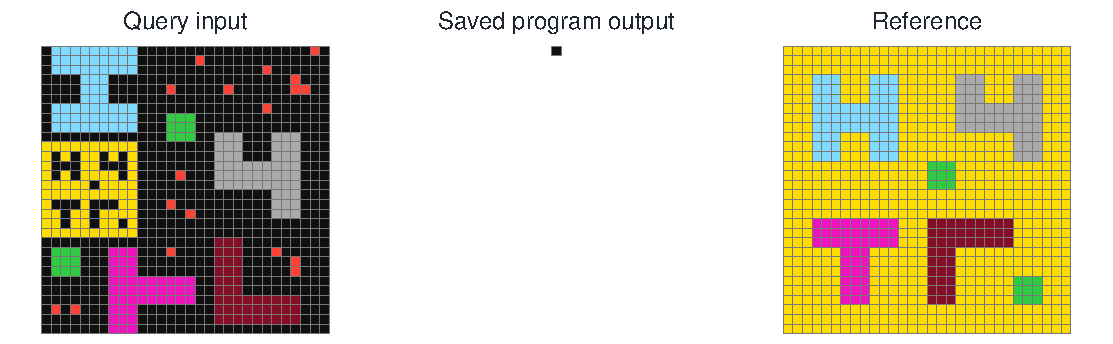
\includegraphics[height=51mm]{python-case-audit/wrong-size.pdf}\end{center}
\med\texttt{out = [[bg] * out\_w for \_ in range(out\_h)]}
\par\vspace{2mm}
The selected component occupied one cell. A returned $1\times1$ for a $30\times30$ reference and missed both demonstrations.
\vfill\smallbody Earlier strict solves on this task: NF4 base 0, checkpoint-660 0, both BF16 samplers 0.
\end{frame}

\begin{frame}[t]{\id{b0039139}\enspace The program handled only row separators}
\med
This was the only wrong task for which a query grid was missing. A looked for all-blue separator rows, then assigned colors from the row groups after the first.
\par\vspace{4mm}
\begin{tabular}{@{}lccc@{}}\toprule
 & Separator direction & Saved result & Reference\\\midrule
Query 1 & Three rows & $12\times1$ & $19\times5$\\
Query 2 & Three columns & No grid & $5\times29$\\
\bottomrule\end{tabular}
\par\vspace{4mm}
The second input contained zero separator rows. The code therefore collected zero colors and reached \texttt{if not colors: return []}. The scoring record has no valid grid for that query.
\vfill\smallbody A matched 0/4 demonstrations. All four NF4/BF16 direct runs missed the task. OpenRouter solved it once in ten trials.
\end{frame}

\begin{frame}[t]{\id{2b83f449}\enspace A condition made every edit impossible}
\med
On three tasks, B returned the query input unchanged. On this one it first required every cell in a $3\times3$ block to be color 7. It then tried to repaint cells within that block only if their original color was 8.
\par\vspace{1mm}
\begin{center}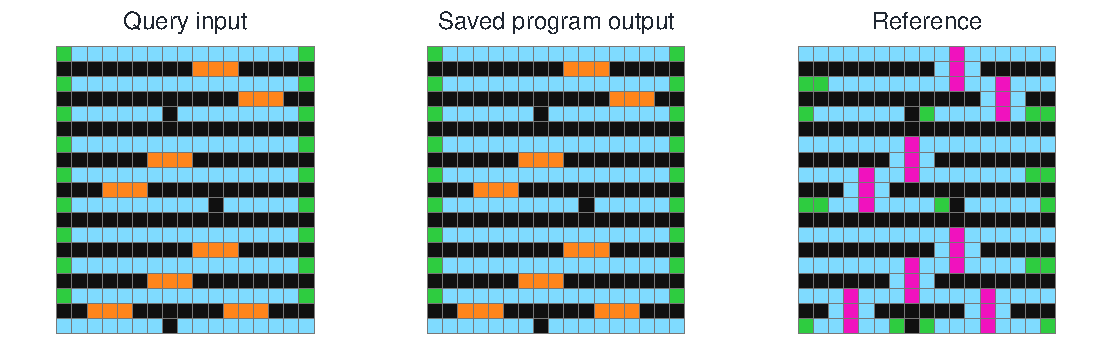
\includegraphics[height=48mm]{python-case-audit/copied.pdf}\end{center}
\med The two conditions cannot hold for the same cell. The output copied all 323 input cells. The reference required 62 changes. The program matched 0/2 demonstrations.
\vfill\smallbody Earlier strict solves on this task: NF4 base 0, checkpoint-660 0, both BF16 samplers 0.
\end{frame}

\begin{frame}[t]{\id{97d7923e}\enspace Correct dimensions, nine incorrect cells}
\med
Four A tasks and five B tasks returned the right dimensions and changed the input, yet missed the reference. Here B scanned each column for a vertical run of 5s between two 2s and repainted it with 2s.
\par\vspace{2mm}
\begin{center}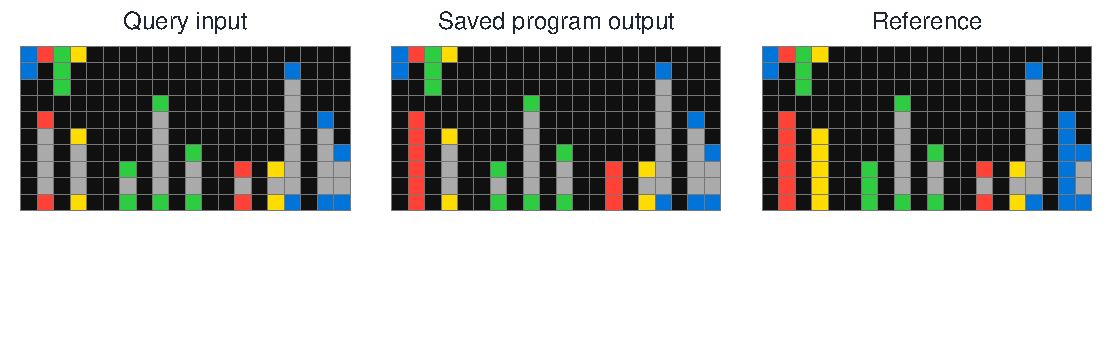
\includegraphics[height=48mm]{python-case-audit/wrong-cells.pdf}\end{center}
\med The result matched 191 of 200 cells. The same rule failed all three demonstrations. One wrong cell suffices to fail exact scoring.
\vfill\smallbody Earlier strict solves on this task: NF4 base 0, checkpoint-660 0, both BF16 samplers 0.
\end{frame}
